\documentclass[11pt,a4paper]{article}
\usepackage[T1]{fontenc}
\usepackage[utf8]{inputenc}
\usepackage{newpxtext}
\usepackage[margin=26mm,headheight=15pt]{geometry}
\usepackage{microtype}
\usepackage{amsmath,amsthm,mathtools}
\usepackage{newpxmath}
\usepackage{booktabs,array,tabularx}
\usepackage{xcolor}
\definecolor{Olive}{HTML}{48573D}
\definecolor{Sage}{HTML}{EDF0E7}
\definecolor{Ink}{HTML}{26302A}
\definecolor{Muted}{HTML}{626960}
\usepackage{enumitem}
\usepackage{needspace}
\setlist{itemsep=3pt,topsep=5pt}
\usepackage[most]{tcolorbox}
\newtcolorbox{resultbox}{colback=Sage,colframe=Olive,boxrule=.6pt,
  arc=1.2mm,left=3mm,right=3mm,top=2mm,bottom=2mm,breakable}
\usepackage{tikz}
\usetikzlibrary{arrows.meta,positioning}
\usepackage{listings}
\lstset{basicstyle=\ttfamily\small,columns=fullflexible,keepspaces=true,
  frame=single,framerule=.3pt,rulecolor=\color{Olive},
  backgroundcolor=\color{Sage},breaklines=true,showstringspaces=false}
\usepackage{fancyhdr}
\pagestyle{fancy}
\fancyhf{}
\fancyhead[L]{\small\color{Muted}Cofinal strata and ordinal absorption}
\fancyhead[R]{\small\color{Muted}Research article}
\fancyfoot[C]{\small\thepage}
\renewcommand{\headrulewidth}{.3pt}
\usepackage{titlesec}
\titleformat{\section}{\Large\bfseries\color{Olive}}{\thesection}{.65em}{}
\titleformat{\subsection}{\large\bfseries\color{Olive}}{\thesubsection}{.65em}{}
\usepackage[colorlinks=true,linkcolor=Olive,citecolor=Olive,urlcolor=Olive,
  pdfauthor={ChatGPT},pdftitle={Cofinal strata and ordinal absorption},
  pdfsubject={Finitary powersets of finite lexicographic sums}]{hyperref}
\usepackage{bookmark}
\usepackage[numbers,sort&compress]{natbib}
\newtheorem{theorem}{Theorem}[section]
\newtheorem{lemma}[theorem]{Lemma}
\newtheorem{proposition}[theorem]{Proposition}
\newtheorem{corollary}[theorem]{Corollary}
\theoremstyle{definition}
\newtheorem{definition}[theorem]{Definition}
\newtheorem{example}[theorem]{Example}
\newtheorem{problem}[theorem]{Problem}
\theoremstyle{remark}
\newtheorem{remark}[theorem]{Remark}
\newcommand{\K}{\mathcal K}
\newcommand{\M}{\mathcal M}
\newcommand{\ot}{\operatorname{o}}
\newcommand{\hgt}{\operatorname{h}}
\newcommand{\wid}{\operatorname{w}}
\newcommand{\ns}{\mathbin{\#}}
\newcommand{\bigns}{\mathop{\#}\limits}
\newcommand{\np}{\mathbin{\otimes}}
\newcommand{\pred}{\operatorname{Pred}}
\newcommand{\supp}{\operatorname{supp}}
\newcommand{\tr}{\operatorname{tr}}
\newcommand{\rk}{\operatorname{rk}}
\newcommand{\eps}{\varepsilon_0}
\newcommand{\N}{\mathbb N}
\newcommand{\Fin}{\operatorname{Fin}}
\newcommand{\lxs}{\mathop{\sum}\limits^{\mathrm{lex}}}
\newcommand{\cR}{\mathcal R}
\allowdisplaybreaks[2]
\emergencystretch=1em
\setlength{\parskip}{3pt}
\setlength{\parindent}{1.2em}

\begin{document}
\hypersetup{pageanchor=false}
\begin{titlepage}
\vspace*{10mm}
{\small\sffamily\color{Olive}ORDER THEORY\quad /\quad ORDINAL COMBINATORICS}
\vspace{12mm}

{\Huge\bfseries\color{Ink}Cofinal strata and\par ordinal absorption\par}
\vspace{6mm}
{\Large Finitary powersets of finite lexicographic sums\par}
\vspace{12mm}
{\large An exploratory research article\par}
{\normalsize Prepared for Vladimir Reshetnikov with ChatGPT\par}
{\normalsize 19 September 2026\par}
\vspace{12mm}

\begin{abstract}
We investigate a concrete instance of the published problem of enlarging
classes of well-quasi-orders whose finitary powersets have compositionally
computable ordinal invariants. For a finite poset $Q$, we stratify the finitely
generated downsets of a lexicographic sum $\sum_{q\in Q}^{\mathrm{lex}}P_q$
by the inclusion-maximal antichains of $Q$. Under explicit hypotheses on the
fibers, each stratum has a pure maximal order type $\omega^{\gamma_A}$.
A cofinal-absorption theorem shows that its contribution survives exactly
when no higher stratum has a strictly larger exponent.

For uniform ordinal fibers $\alpha=\omega^\rho$, $\rho>0$, this yields
\[
 \ot\bigl(\K(S_\alpha(Q))\bigr)
   =\sum_{k=\wid(Q)}^{1}\omega^{\rho\np k}c_k(Q),
 \qquad
 \hgt\bigl(\K(S_\alpha(Q))\bigr)
   =\alpha\cdot\hgt(\M(Q)).
\]
Here $c_k(Q)$ counts maximal antichains of size $k$ not dominated by a larger
one, and $\M(Q)$ is their domination poset. The first formula extends to
nonuniform WPO fibers of prescribed pure finitary-powerset type. We also
obtain a leading-coefficient counting reduction, an explicit maximal-chain
construction, and a Cantor-normal-form truncation rule for finite
nonuniform lexicographic sums. Complete proofs accompany exact-arithmetic
Python code and finite structural checks. This is a partial answer to the
broader research direction, not a solution of its general width or
arbitrary-iteration problems; priority of the derived formulas is not
independently established.
\end{abstract}
\vfill
\begin{resultbox}
\small\textbf{Scope of the claims.} The mathematical results below are proved
from stated standard WPO facts. The accompanying computations test finite
identities and the implementation; they are not a formal verification of
infinite ordinals. The general extension question remains broader than the
class treated here.
\end{resultbox}
\end{titlepage}
\pagenumbering{roman}
\hypersetup{pageanchor=true}
\setcounter{tocdepth}{1}
\hypersetup{bookmarksdepth=2}
\tableofcontents
\newpage
\pagenumbering{arabic}

\section{The selected open direction and the precise target}

Abriola, Halfon, Lopez, Schmitz, Schnoebelen and Vialard ask, in the conclusion
of \emph{Measuring well-quasi-ordered finitary powersets}, which extensions
of their elementary family retain computable ordinal invariants
\cite[Section 6, p.~23]{AbriolaEtAl2024}. Their grammar uses disjoint unions,
Cartesian products, words, multisets and finitary powersets. Arbitrary
finite-poset lexicographic gluing is not one of its constructors. We take
this missing constructor as a specific target.

\begin{problem}[Finite-gluing instance]\label{prob:target}
Let $Q$ be a finite poset and let $P_q$, $q\in Q$, be WPOs. Determine the
maximal order type and height of the finitary powerset of
\[
 S=\lxs_{q\in Q}P_q,
\]
from finite information about $Q$ and appropriate invariants of the fibers.
In particular, obtain exact formulas when every fiber is the ordinal
$\omega^\rho$, for a fixed $\rho>0$.
\end{problem}

This formulation is our concrete subproblem, not a quotation of a separately
numbered conjecture. The broad published question does not prescribe this
particular class. The results here give an additional compositional rule
with explicit hypotheses, rather than a claim that the whole elementary
calculus has been closed under a new operation.

\subsection{What is established here}

The general maximal-order-type result is Theorem~\ref{thm:general}. Its
hypotheses require that the fibers have no finite cofinal subsets and that
$\ot(\K(P_q))=\omega^{\beta_q}$, with $\beta_q>0$. The exponents may vary
with $q$, and the fibers need not be chains. The two uniform formulas are
Corollary~\ref{cor:uniform} and Theorem~\ref{thm:height}. The latter includes
an actual chain attaining the computed height.

The main proof mechanism is independent of finitary powersets: a finite
stratification with pure stratum types and upward cofinality admits an
exact survivor formula. The finitary-powerset construction supplies a
canonical such stratification. The distinction between a finite
stratification and a lexicographic decomposition is essential: comparable
strata need not have all their points comparable.

We do not determine ordinal width in general. Nor do we claim a formula
for arbitrary repeated applications of $\K$, arbitrary impure fiber types,
or infinite indexing posets. A concrete failure of a tempting nonuniform
height formula is proved in Section~\ref{sec:boundaries}.

\subsection{Status and relation to existing results}

The source for the open direction is the July 2024 version of
\cite{AbriolaEtAl2024}; its arXiv record and the final-page question were
checked on 19 September 2026. A targeted literature search did not locate
the frontier formulas proved below. That search is not a proof of novelty,
and the results should be checked against specialist literature before
priority is claimed.

A nearby problem must not be confused with our target: maximal order types
of uniform lexicographic products have already been treated in Vialard's
published 2025 paper \cite{Vialard2025}. We use that publication, rather
than an older preprint's status statement, in assessing the literature.
Appendix~\ref{sec:lex} derives a finite nonuniform formula as a supporting
result and recovers the known finite uniform case. It is not presented as
a resolution of an open lexicographic-product problem.

The background facts about maximal linearizations and natural operations
are classical \cite{deJonghParikh1977,DSS2020}. The contribution attempted
here is the cofinal-stratum reduction and its consequences for the chosen
finite-gluing instance.

\section{Definitions and ordinal tools}\label{sec:tools}

\subsection{WPOs, rank and maximal order type}

A \emph{well-partial-order} (WPO) is a partial order in which every infinite
sequence $x_0,x_1,\ldots$ has $i<j$ with $x_i\le x_j$. All posets considered
below are sets, and we work in ordinary set theory with choice. A
well-quasi-order can be replaced by its quotient under mutual comparison.

A \emph{linearization} is a total order extending the partial order on the
same underlying set. Every linearization of a WPO is a well-order. Its
largest possible order type is denoted $\ot(P)$. The de Jongh--Parikh
maximal-linearization theorem guarantees that this maximum is attained
\cite{deJonghParikh1977}.

For a well-founded poset, define
\[
 r_P(x)=\sup_{y<x}\bigl(r_P(y)+1\bigr),
 \qquad
 \hgt(P)=\sup_{x\in P}\bigl(r_P(x)+1\bigr).
\]
We use $\hgt(\varnothing)=0$. This is the height defined by the rank of the
tree of finite strictly decreasing sequences. In particular, an ordinal
chain $\alpha$ has height $\alpha$. An order-preserving rank bound will
mean a map into ordinals which is \emph{strictly} increasing on strict
comparisons; such a map bounds $r_P$ pointwise by well-founded induction.

The ordinal width $\wid(P)$ is the rank of the tree of finite sequences of
pairwise incomparable elements. When $P$ has finite maximum antichain
cardinality $d$, this ordinal width equals the integer $d$. We use width
only in this finite sense for index posets and the input examples; no
general output-width formula is asserted.

\subsection{Finite downsets and the Hoare quotient}

For a poset $P$, set
\[
 \K(P)=\{\downarrow F:F\subseteq P\text{ finite}\},
 \qquad
 \downarrow F=\{x\in P:\exists f\in F\ (x\le f)\},
\]
ordered by inclusion. The empty set belongs to $\K(P)$. Finite subsets have
the Hoare relation
\[
 F\le_H G\quad\Longleftrightarrow\quad
 (\forall f\in F)(\exists g\in G)\ f\le g.
\]
This is equivalent to $\downarrow F\subseteq\downarrow G$, so $\K(P)$ is
exactly its antisymmetric quotient. These are finitely generated
\emph{downsets}; they are not required to be directed ideals. Equivalently,
they are the compact elements of the lattice of all downsets of $P$.

For a WPO $P$, $\K(P)$ is a WPO. One standard proof applies the finite-word
WPO theorem to arbitrary enumerations of finite subsets: a word embedding
implies Hoare domination. We write
$\K(P)^+=\K(P)\setminus\{\varnothing\}$.

A subset $C\subseteq P$ is \emph{cofinal} if every $p\in P$ satisfies
$p\le c$ for some $c\in C$. Thus
\begin{equation}\label{eq:nofinite}
 P\text{ has no finite cofinal subset}
 \quad\Longleftrightarrow\quad P\notin\K(P).
\end{equation}
This condition ensures that a whole fiber cannot be generated internally
by finitely many points.

\subsection{Lexicographic sums}

For pairwise disjoint nonempty posets $P_q$ indexed by a finite poset $Q$,
write $S=\sum_{q\in Q}^{\mathrm{lex}}P_q$. Within a fiber we use its original
order; for different fibers all points of $P_q$ lie below all points of
$P_r$ exactly when $q<r$. Fibers over incomparable indices remain
incomparable. The resulting poset is a WPO whenever every fiber is a WPO:
an infinite sequence has an infinite subsequence in a single fiber.

For uniform ordinal fibers $P_q=\alpha$, denote this poset by
$S_\alpha(Q)$. This notation avoids choosing between competing conventions
for the order of factors in a lexicographic product.

\subsection{Natural arithmetic and standard monotonicity}

Unmarked $+$ and $\cdot$ are ordinary ordinal addition and multiplication.
We use $\ns$ for Hessenberg natural sum and $\np$ for natural product. In
Cantor normal form, natural sum adds coefficients at equal exponents;
natural product multiplies the corresponding formal polynomials, using
natural sum for exponents. Consequently
\begin{equation}\label{eq:pureproduct}
 \omega^\beta\np\omega^\gamma=\omega^{\beta\ns\gamma},
 \qquad
 \underbrace{\rho\ns\cdots\ns\rho}_{k\text{ times}}=\rho\np k.
\end{equation}
Natural sum is strictly increasing in each argument. For any $\beta$,
\begin{equation}\label{eq:closure}
 \mu_1,\ldots,\mu_t<\omega^\beta
 \quad\Longrightarrow\quad
 \mu_1\ns\cdots\ns\mu_t<\omega^\beta
\end{equation}
when $t$ is finite. For $\beta=0$, all the $\mu_i$ are zero. For $\beta>0$,
this follows immediately from the finite Cantor normal forms: every
appearing exponent is below $\beta$.

We use the following standard WPO facts
\cite{deJonghParikh1977,DSS2020}:
\begin{equation}\label{eq:standard}
 \ot(P\sqcup R)=\ot(P)\ns\ot(R),
 \qquad
 \ot(P\times R)=\ot(P)\np\ot(R).
\end{equation}
An induced subposet cannot have larger maximal order type. Adding
comparisons on the same set cannot increase maximal order type, because it
only removes possible linearizations. It follows that, for a finite
partition $P=\bigsqcup_i P_i$ into induced subposets,
\begin{equation}\label{eq:partitionbound}
 \ot(P)\le\bigns_i\ot(P_i).
\end{equation}
These background results are the nontrivial external inputs to our proofs.
The new reductions below do not assume a general formula for the
finitary-powerset operation.

\section{Cofinal absorption}\label{sec:absorption}

The first lemma explains why certain low-exponent strata can disappear
entirely from a maximal order type.

\begin{lemma}[Cofinal absorption]\label{lem:absorption}
Let $X$ be a WPO with a disjoint partition $X=U\sqcup V$. Suppose that $U$
is cofinal in $X$ and
\[
 \ot(U)=\kappa=\omega^\beta,
 \qquad \ot(V)<\kappa.
\]
Then $\ot(X)=\kappa$.
\end{lemma}

\begin{proof}
The lower bound follows because $U$ is an induced subposet of $X$.
For the upper bound, let $L$ be any linearization of $X$. Suppose its order
type is greater than $\kappa$. Let $I$ be its initial segment consisting of
the first $\kappa$ positions.

The restriction of $L$ to $U\cap I$ has order type at most $\kappa$.
If it had type $\mu<\kappa$, the restriction to $V\cap I$ would have some
type $\nu\le\ot(V)<\kappa$. The order $I$ is a linearization of the
disjoint union of these two restricted well-orders. Hence
\[
 \kappa=\operatorname{type}(I)\le\mu\ns\nu<\kappa,
\]
by \eqref{eq:standard} and \eqref{eq:closure}, a contradiction. Therefore
$L\upharpoonright(U\cap I)$ has type exactly $\kappa$.

Choose $x$ at a position after $I$. Cofinality gives $u\in U$ with $x\le u$.
Since $L$ extends $X$, $u$ also occurs after $I$. Thus $L\upharpoonright U$
contains its initial suborder of type $\kappa$ and another point after it,
so its type is at least $\kappa+1$. This contradicts $\ot(U)=\kappa$.
No linearization can exceed $\kappa$, proving the result.
\end{proof}

Cofinality alone is insufficient when the cofinal part has an impure
maximal type. For example, let $U$ have type $\omega+1$, let $v$ be
incomparable with the initial $\omega$ points of $U$, and put $v$ below its
last point. Then $U$ is cofinal but $\ot(U\cup\{v\})=\omega+2$.
The pure-power assumption in Lemma~\ref{lem:absorption} is doing real work.

\section{A finite cofinal-stratification theorem}\label{sec:stratification}

\begin{definition}
A \emph{finite cofinal stratification} of a WPO $X$ consists of a finite
poset $I$ and a partition $X=\bigsqcup_{i\in I}X_i$ into nonempty induced
subposets such that
\begin{align}
 x\in X_i,\,y\in X_j,\ x\le y&\ \Longrightarrow\ i\le j,
       \label{eq:indexrespect}\\
 i\le j&\ \Longrightarrow\
 (\forall x\in X_i)(\exists y\in X_j)\ x\le y.
       \label{eq:upcofinal}
\end{align}
The second condition is upward cofinality, not universal comparability.
\end{definition}

\begin{theorem}[Surviving strata]\label{thm:strata}
Suppose $X=\bigsqcup_{i\in I}X_i$ has a finite cofinal stratification and
$\ot(X_i)=\omega^{\beta_i}$. Define
\[
 R=\{i\in I:\text{there is no }j>i\text{ with }\beta_j>\beta_i\}.
\]
Then
\begin{equation}\label{eq:strataformula}
 \boxed{\displaystyle \ot(X)=\bigns_{i\in R}\omega^{\beta_i}.}
\end{equation}
Moreover, some maximal linearization places each entire stratum in a
single block.
\end{theorem}

\begin{proof}
\emph{Upper bound.} For each $i\notin R$, choose $r(i)\ge i$ for which
$\beta_{r(i)}$ is maximal among the exponents of successors of $i$,
including $i$ itself. Since $i$ is not a survivor, this maximum is strictly
larger than $\beta_i$. Furthermore, $r(i)\in R$: a successor of $r(i)$ with
still larger exponent would contradict its choice.

For each $r\in R$, form the induced subposet
\[
 G_r=X_r\ \cup\!\!\bigcup_{\{i\notin R:r(i)=r\}}X_i.
\]
These groups partition $X$. By upward cofinality, $X_r$ is cofinal in
$G_r$. By the partition bound and finite natural-sum closure,
\[
 \ot(G_r\setminus X_r)
 \le\bigns_{\{i:r(i)=r\}}\omega^{\beta_i}
 <\omega^{\beta_r}.
\]
The inequality also holds when the group has no other strata, since the
left side is zero. Lemma~\ref{lem:absorption} yields
$\ot(G_r)=\omega^{\beta_r}$. Applying the partition bound once more proves
$\ot(X)\le\bigns_{r\in R}\omega^{\beta_r}$.

\emph{Lower bound.} If $i,j\in R$ and $i<j$, then $\beta_i\ge\beta_j$;
otherwise $i$ would not survive. Order the elements of $R$ by
nonincreasing exponent, breaking ties by any linear extension of their
induced order. This total order is compatible with the order inherited
from $I$.

Any linear extension of an induced subposet of a finite poset extends to a
linear extension of the whole poset. To see this directly, add the chosen
comparisons between elements of the subposet. A directed cycle would give
a chain of newly added comparisons, linked by old directed paths, whose
endpoints lie in the subposet. Each old path already induces a comparison
in its inherited order. Such a cycle would contradict compatibility of
the chosen total order. The enlarged acyclic relation therefore has a
linear extension.

Apply this observation to $R\subseteq I$. Concatenate maximal
linearizations of all the $X_i$ in the resulting order of $I$. Condition
\eqref{eq:indexrespect} ensures that this concatenation is a linearization
of $X$. Its restriction to survivor blocks is an ordinary sum of the
monomials $\omega^{\beta_i}$ in nonincreasing exponent order. That ordinary
sum equals their natural sum. The entire linearization has at least this
order type, giving the lower bound. The upper bound already proved shows
that the concatenation is maximal.
\end{proof}

\begin{remark}
The theorem permits repeated exponents. A higher stratum of \emph{equal}
exponent does not absorb a lower one; both contributions survive unless a
strictly larger exponent occurs still higher. This strict inequality is
responsible for the finite coefficients in later formulas.
\end{remark}

The proof also explains why an algorithm considering only block orders is
not by itself enough. Such an algorithm supplies a lower bound. The
cofinal-absorption argument controls all possible interleavings inside
linearizations and supplies the matching upper bound.

\section{The frontier poset of a finite order}\label{sec:frontiers}

\begin{definition}
For a nonempty finite poset $Q$, let $\M(Q)$ be its set of
\emph{inclusion-maximal} antichains. For $A\in\M(Q)$ put
\[
 D(A)=\{q\in Q:\exists a\in A\ (q<a)\}.
\]
Order maximal antichains by domination:
\begin{equation}\label{eq:frontierorder}
 A\preceq B\quad\Longleftrightarrow\quad
 (\forall a\in A)(\exists b\in B)\ a\le b.
\end{equation}
We call $(\M(Q),\preceq)$ the \emph{frontier poset}.
\end{definition}

Maximality here is by inclusion, not cardinality. A maximal antichain can
have fewer elements than the width of $Q$. This is exactly what happens
in the two orientations of a three-point fork.

\begin{lemma}\label{lem:frontiers}
For $A,B\in\M(Q)$,
\begin{equation}\label{eq:frontierD}
 A=\min(Q\setminus D(A)),
 \qquad
 A\preceq B\ \Longleftrightarrow\ D(A)\subseteq D(B).
\end{equation}
In particular, $A\mapsto D(A)$ is injective and $\preceq$ is a partial
order. The least and greatest frontiers are $\min Q$ and $\max Q$.
\end{lemma}

\begin{proof}
Every predecessor of an element of $A$ lies in $D(A)$, while $A$ itself is
disjoint from $D(A)$. Conversely, suppose $x\in\min(Q\setminus D(A))$.
By maximality, $x$ is comparable with an element $a\in A$. It cannot lie
strictly below $a$, since then $x\in D(A)$. It cannot lie strictly above
$a$, since $a\notin D(A)$ would contradict minimality of $x$. Thus $x=a$.

If $A\preceq B$, every strict predecessor of an $a\in A$ is a strict
predecessor of some $b\in B$, proving $D(A)\subseteq D(B)$. Conversely,
assume this inclusion and take $a\in A$. If $a\in D(B)$, it is strictly
below some $b\in B$. Otherwise every strict predecessor of $a$ lies in
$D(A)\subseteq D(B)$, so $a\in\min(Q\setminus D(B))=B$. Either way $a$
is dominated by $B$.

Injectivity follows from the first identity. Every element of a finite
poset lies above a minimal element and below a maximal one, giving the
last assertion.
\end{proof}

For the $N$-shaped poset with comparisons $a<c$, $b<c$, $b<d$, the
frontiers form the three-element chain
\begin{equation}\label{eq:Nfrontiers}
 \{a,b\}\prec\{a,d\}\prec\{c,d\}.
\end{equation}
The middle frontier is not a level of the original height-two poset.
This already suggests why its finitary powerset can have three ordinal
height stages rather than two.

\begin{figure}[htbp]
\centering
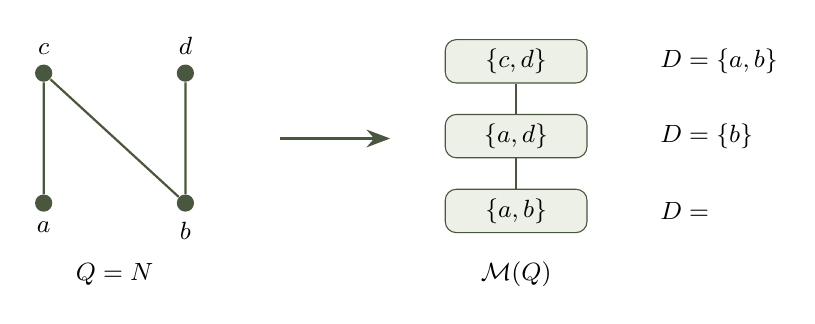
\begin{tikzpicture}[every node/.style={font=\small},
 dot/.style={circle,fill=Olive,inner sep=2.2pt}]
 \node[dot,label=below:$a$] (a) at (0,0) {};
 \node[dot,label=below:$b$] (b) at (1.8,0) {};
 \node[dot,label=above:$c$] (c) at (0,1.65) {};
 \node[dot,label=above:$d$] (d) at (1.8,1.65) {};
 \draw[Olive,thick] (a)--(c) (b)--(c) (b)--(d);
 \node at (.9,-.9) {$Q=N$};
 \draw[-{Stealth[length=3mm]},thick,Olive] (3,.82)--(4.4,.82);
 \node[draw=Olive,rounded corners,fill=Sage,minimum width=18mm] (A) at (6,-.1)
      {$\{a,b\}$};
 \node[draw=Olive,rounded corners,fill=Sage,minimum width=18mm] (B) at (6,.85)
      {$\{a,d\}$};
 \node[draw=Olive,rounded corners,fill=Sage,minimum width=18mm] (C) at (6,1.8)
      {$\{c,d\}$};
 \draw[Olive,thick] (A)--(B)--(C);
 \node[right=8mm of A] {$D=\varnothing$};
 \node[right=8mm of B] {$D=\{b\}$};
 \node[right=8mm of C] {$D=\{a,b\}$};
 \node at (6,-.9) {$\M(Q)$};
\end{tikzpicture}
\caption{A height-two skeleton can have a height-three frontier poset.
The right-hand labels are the completed-fiber sets.}
\label{fig:N}
\end{figure}

\section{Canonical strata of the finitary powerset}\label{sec:canonical}

Let $S=\sum_{q\in Q}^{\mathrm{lex}}P_q$, where $Q$ is finite and nonempty,
and assume that every nonempty fiber $P_q$ has no finite cofinal subset.
For $K\in\K(S)$ define its set of \emph{completed fibers} by
\[
 D_K=\{q\in Q:P_q\subseteq K\}.
\]

\begin{lemma}[Canonical frontier]\label{lem:canonical}
Every $K\in\K(S)$ has a unique frontier $A\in\M(Q)$ with $D_K=D(A)$.
For this frontier, $K$ contains all of each fiber indexed by $D(A)$,
intersects fibers indexed by $A$ in finitely generated downsets, and is
empty on all other fibers.
\end{lemma}

\begin{proof}
Write $K=\downarrow F$ with $F$ finite, let $B$ be the set of indices
meeting $F$, and let $A_0=\max B$. For $F=\varnothing$, take
$B=A_0=\varnothing$.

If $q<a$ for some $a\in A_0$, a generator in $P_a$ lies above every point
of $P_q$, so $P_q\subseteq K$. If no generator has index strictly above
$q$, then $K\cap P_q$ is generated internally by the finite set
$F\cap P_q$. By \eqref{eq:nofinite}, it cannot be all of $P_q$. Therefore
\begin{equation}\label{eq:Dsupport}
 D_K=D(A_0)=\bigcup_{a\in A_0}\{q:q<a\}.
\end{equation}
Write this downset as $D$ and put $A=\min(Q\setminus D)$. Every member of
$A_0$ belongs to $A$: its predecessors lie in $D$, and it does not lie in
$D$ itself. Conversely, every strict predecessor of an element of $A$
lies in $D$. Thus $D(A)=D$, since $D=D(A_0)\subseteq D(A)$ as well.

The set $A$ is a maximal antichain. An element outside $D$ lies above a
minimal element of $Q\setminus D$, while an element of $D$ lies below
some member of $A_0\subseteq A$. Thus every element of $Q$ is comparable
with a member of $A$.

A nonempty intersection $K\cap P_q$ with $q\notin D$ requires a generator
at index $q$ itself, with no generator strictly above it. Hence
$q\in A_0\subseteq A$. These intersections are generated by $F\cap P_q$.
The uniqueness of $A$ follows from Lemma~\ref{lem:frontiers}.
\end{proof}

Let $X_A$ be the set of all $K\in\K(S)$ with completed-fiber set $D(A)$.
For $a\in A$, write $K_a=K\cap P_a$. The lemma gives a precise product
representation, with one support condition:
\begin{equation}\label{eq:tuplecondition}
 X_A\ \cong\
 \left\{(K_a)_{a\in A}\in\prod_{a\in A}\K(P_a):
 D(A)=\bigcup_{\{a:K_a\ne\varnothing\}}\{q:q<a\}\right\}.
\end{equation}
The order is coordinatewise inclusion. To verify sufficiency, choose
finite generators for the nonempty $K_a$ and take their union inside $S$.
The support condition makes its completed-fiber set exactly $D(A)$.
Necessity follows from \eqref{eq:Dsupport}.

In particular, as induced subposets,
\begin{equation}\label{eq:sandwich}
 \prod_{a\in A}\K(P_a)^+
 \ \subseteq\ X_A\ \subseteq\ \prod_{a\in A}\K(P_a).
\end{equation}
Every $X_A$ is nonempty, since all active coordinates can be chosen
nonempty. The empty downset belongs to the stratum indexed by $\min Q$;
there is no extra empty stratum.

\begin{lemma}[Cofinal frontier stratification]\label{lem:cofinalfrontier}
The partition
\[
 \K(S)=\bigsqcup_{A\in\M(Q)}X_A
\]
is a finite cofinal stratification indexed by $\M(Q)$.
\end{lemma}

\begin{proof}
If $K\subseteq L$, every fiber completed by $K$ is completed by $L$.
Thus $D_K\subseteq D_L$, and Lemma~\ref{lem:frontiers} gives the required
comparison of frontier indices.

For upward cofinality, let $A\preceq B$ and $K\in X_A$. Choose nonempty
finitely generated downsets $L_b\in\K(P_b)^+$ for every $b\in B$. When
$b\in A\cap B$, choose $L_b$ to contain $K_b$: adjoin one point to its
finite generating set if necessary. Use these coordinates and completed
fibers $D(B)$ to form $L\in X_B$.

We have $D(A)\subseteq D(B)$. Moreover, each $a\in A\setminus B$ lies
strictly below some $b\in B$, so its entire fiber is completed in $L$.
The remaining active coordinates, indexed by $A\cap B$, were explicitly
enlarged. Hence $K\subseteq L$.
\end{proof}

The last argument chooses $L$ in response to $K$. It does not say that
\emph{every} member of $X_B$ dominates $K$. For example, for the skeleton
consisting of an isolated point $x$ and a chain $y<z$, the frontiers
$\{x,y\}\prec\{x,z\}$ share an $x$-coordinate. A downset with a large
$x$-coordinate in the first stratum is not below one with a small
$x$-coordinate in the second. This is why replacing the strata by fully
ordered blocks would give only a bound without Theorem~\ref{thm:strata}.

\section{The general maximal-order-type formula}\label{sec:general}

\begin{lemma}[Removing the least downset]\label{lem:removebottom}
If $\ot(\K(P))$ is infinite, then
$\ot(\K(P)^+)=\ot(\K(P))$.
\end{lemma}

\begin{proof}
The empty downset is below everything else, so every linearization is a
single least point followed by a linearization of $\K(P)^+$. Attainment
of maximal linearizations gives
$\ot(\K(P))=1+\ot(\K(P)^+)$. The latter type must be infinite; for every
infinite ordinal $\eta$, $1+\eta=\eta$.
\end{proof}

\begin{remark}[Purity already excludes finite cofinality]
In the next theorem the no-finite-cofinality assumption is stated to make
the structural argument visible, but it follows from the positive pure
type assumption. Indeed, a finite cofinal subset of $P$ would make $P$
itself the greatest member of $\K(P)$. Then
\[
 \ot(\K(P))=\ot(\K(P)\setminus\{P\})+1
\]
would be a successor ordinal, whereas $\omega^\beta$ is a limit for
$\beta>0$. Thus the numerical hypothesis alone implies this boundary
condition (and also implies that $P$ is nonempty).
\end{remark}

\begin{samepage}
\begin{theorem}[Finite lexicographic gluing]\label{thm:general}
Let $Q$ be a finite nonempty poset. For each $q\in Q$, let $P_q$ be a
nonempty WPO having no finite cofinal subset and satisfying
\[
 \ot(\K(P_q))=\omega^{\beta_q},\qquad \beta_q>0.
\]
For $A\in\M(Q)$ define
\[
 \gamma_A=\bigns_{a\in A}\beta_a,
 \qquad
 \cR=\{A\in\M(Q):\nexists B\succ A\ (\gamma_B>\gamma_A)\}.
\]
Then
\begin{equation}\label{eq:main}
 \boxed{\displaystyle
 \ot\left(\K\left(\lxs_{q\in Q}P_q\right)\right)
   =\bigns_{A\in\cR}\omega^{\gamma_A}.}
\end{equation}
\end{theorem}
\end{samepage}

\begin{proof}
For each frontier $A$, the two outer products in \eqref{eq:sandwich} have
the same maximal order type, by Lemma~\ref{lem:removebottom} and the
Cartesian-product formula:
\[
 \mathop{\bigotimes}_{a\in A}\omega^{\beta_a}
   =\omega^{\bigns_{a\in A}\beta_a}=\omega^{\gamma_A}.
\]
Induced-subposet monotonicity therefore gives
$\ot(X_A)=\omega^{\gamma_A}$. Lemma~\ref{lem:cofinalfrontier} provides a
finite cofinal stratification. Apply Theorem~\ref{thm:strata}.
\end{proof}

The theorem is compositional in a precise, limited sense. Once the pure
values $\ot(\K(P_q))$ are known and the no-finite-cofinality hypotheses are
verified, no additional internal data about the fibers enter the output
maximal order type. All remaining work takes place in the finite weighted
frontier poset. This does not supply a method for discovering the required
fiber values for arbitrary input WPOs.

\begin{example}[A nonuniform weighted frontier]
Take the $N$-poset from \eqref{eq:Nfrontiers} and put
\[
 (\beta_a,\beta_b,\beta_c,\beta_d)=(3,1,1,2).
\]
The successive frontier exponents are $4,5,3$. The first is absorbed by
the second, while the second and third survive. Therefore
\[
 \ot\bigl(\K(S)\bigr)=\omega^5+\omega^3.
\]
This is realized, for example, by the ordinal fibers
$(\omega^3,\omega,\omega,\omega^2)$.
\end{example}

\section{Uniform ordinal fibers: an ordinal polynomial}\label{sec:uniform}

Fix $\rho>0$ and $\alpha=\omega^\rho$. Finitely generated downsets of the
chain $\alpha$ are the empty set and principal downsets $\downarrow\xi$
for $\xi<\alpha$. Thus
\begin{equation}\label{eq:ordinalK}
 \K(\alpha)\cong 1+\alpha\cong\alpha.
\end{equation}
The ordinal $\alpha$ is a nonzero limit and has no finite cofinal subset.
All hypotheses of Theorem~\ref{thm:general} hold with $\beta_q=\rho$.

Define the nonnegative integers
\begin{equation}\label{eq:ck}
 c_k(Q)=\#\{A\in\M(Q):|A|=k\text{ and }
                 (\forall B\succeq A)\ |B|\le k\}.
\end{equation}
The notation $\#$ outside ordinal operations in this display denotes
ordinary finite cardinality. In words, $c_k(Q)$ counts size-$k$ maximal
antichains not dominated by a larger maximal antichain.

\begin{corollary}[Uniform maximal order type]\label{cor:uniform}
For a finite nonempty poset $Q$ of width $W$ and $\alpha=\omega^\rho$,
$\rho>0$,
\begin{equation}\label{eq:uniform}
 \boxed{\displaystyle
 \ot\bigl(\K(S_\alpha(Q))\bigr)
   =\omega^{\rho\np W}\cdot c_W(Q)
      +\omega^{\rho\np(W-1)}\cdot c_{W-1}(Q)
      +\cdots+\omega^\rho\cdot c_1(Q).}
\end{equation}
Terms with zero coefficients are omitted. The displayed additions and
coefficient multiplications are ordinary ordinal operations.
\end{corollary}

\begin{proof}
The exponent of a frontier is $\rho\np|A|$, by
\eqref{eq:pureproduct}. Since $\rho>0$, this is strictly increasing with
the positive integer $|A|$. Therefore a frontier survives precisely under
the condition in \eqref{eq:ck}. Collect equal exponents in
Theorem~\ref{thm:general} and list them in decreasing order.
\end{proof}

For $\rho=1$, the output is literally a finite Cantor-normal-form polynomial
in $\omega$ whose coefficients depend on the finite skeleton:
\[
 \ot\bigl(\K(S_\omega(Q))\bigr)
       =\sum_{k=W}^{1}\omega^k c_k(Q).
\]
Thus the infinite ordinal calculation separates into a finite combinatorial
statistic and an explicit substitution in ordinal arithmetic.

\begin{corollary}[Leading coefficient]\label{cor:leading}
The coefficient $c_W(Q)$ is the number of antichains of $Q$ having maximum
cardinality $W$.
\end{corollary}
\begin{proof}
Every maximum-cardinality antichain is inclusion-maximal, and none can be
dominated by an antichain of larger cardinality. Conversely, every
frontier counted by $c_W$ has cardinality $W$.
\end{proof}

\begin{remark}[Natural multiplication cannot be replaced]
For $\rho=\omega+1$ and a two-point antichain $Q$,
\[
 \rho\np2=\omega\cdot2+2,
 \qquad \rho\cdot2=\omega\cdot2+1.
\]
Consequently the maximal order type is
$\omega^{\omega\cdot2+2}$, not $\omega^{\omega\cdot2+1}$.
The code keeps these two multiplication operations separate.
\end{remark}

\section{Exact height and an attaining chain}\label{sec:height}

Let
\[
 \ell(Q)=\hgt(\M(Q)),
\]
where height of the finite frontier poset means the largest number of
elements in one of its chains.

\begin{samepage}
\begin{theorem}[Uniform height]\label{thm:height}
If $Q$ is finite and nonempty and $\alpha=\omega^\rho$ with $\rho>0$, then
\begin{equation}\label{eq:height}
 \boxed{\displaystyle
 \hgt\bigl(\K(S_\alpha(Q))\bigr)=\alpha\cdot\ell(Q).}
\end{equation}
There is a chain of this exact order type inside $\K(S_\alpha(Q))$.
\end{theorem}
\end{samepage}

\begin{proof}
\emph{Upper bound.} Choose an order isomorphism
$\theta:\K(\alpha)\to\alpha$ from \eqref{eq:ordinalK}. For a frontier $A$,
let $d(A)$ be the largest number of strict steps in a chain ending at $A$
in $\M(Q)$. Then $0\le d(A)<\ell(Q)$, and $A\prec B$ implies
$d(A)<d(B)$.

For $K\in X_A$, define
\[
 t_A(K)=\bigns_{a\in A}\theta(K_a),
 \qquad
 R(K)=\alpha\cdot d(A)+t_A(K).
\]
All coordinates $\theta(K_a)$ are below $\alpha$, so finite natural-sum
closure gives $t_A(K)<\alpha$. Thus $R(K)<\alpha\cdot\ell(Q)$.

If $K\subsetneq L$ lie in the same stratum, their active coordinate tuples
are strictly ordered componentwise. Strict monotonicity of natural sum
gives $t_A(K)<t_A(L)$. If their frontiers are distinct, say $A\prec B$,
then
\[
 R(K)<\alpha\cdot(d(A)+1)
       \le\alpha\cdot d(B)\le R(L).
\]
The index-respecting property rules out all other cases. Hence $R$ is
strictly increasing on strict inclusion, so well-founded induction yields
$r_{\K(S)}(K)\le R(K)$. Since $R(K)<\alpha\cdot\ell(Q)$ for every $K$,
the definition of height gives the required upper bound.

\emph{Lower bound and attainment.} Choose a longest frontier chain
\[
 A_0\prec A_1\prec\cdots\prec A_{\ell-1},
 \qquad \ell=\ell(Q).
\]
For each $i<\ell-1$, choose $a_i\in A_i\setminus A_{i+1}$. Such a point
exists: if one inclusion-maximal antichain were properly contained in
another, it would not be maximal. Since $A_i\preceq A_{i+1}$ and
$a_i\notin A_{i+1}$, we have $a_i\in D(A_{i+1})$. It belongs to every
later completed-fiber set as well. At the last stage choose any
$a_{\ell-1}\in A_{\ell-1}$.

For each $i$ and $\xi<\alpha$, form $K_{i,\xi}\in X_{A_i}$ by completing
all fibers in $D(A_i)$, setting every active coordinate other than $a_i$
to $\downarrow0$, and setting the $a_i$-coordinate to $\downarrow\xi$.
Every active coordinate is nonempty, so these are valid members of the
stratum. For fixed $i$, the family $(K_{i,\xi})_{\xi<\alpha}$ is a chain
of type $\alpha$.

If $i<j$, the varying coordinate $a_i$ is completed at stage $j$. Any
other coordinate in $A_i$ is either completed at stage $j$ or remains an
active coordinate there, whose downset contains $\downarrow0$. Already
completed fibers stay completed. It follows that
$K_{i,\xi}\subseteq K_{j,\eta}$ for all $\xi,\eta<\alpha$. Inclusion is
strict because $D(A_i)\subsetneq D(A_j)$: some fiber is fully present at
stage $j$ but not at stage $i$.

The ordered concatenation of these $\ell$ many chains is therefore a
chain of type $\alpha\cdot\ell$. This proves the lower bound and
attainment.
\end{proof}

The height and maximal-order-type formulas inspect different aspects of
the same finite object. Height records the longest chain of frontiers.
Maximal order type records the exponents of frontiers that cannot be
absorbed from above. Neither statistic determines the other.

\section{Examples and comparisons}\label{sec:examples}

\subsection{Chains, antichains and oriented forks}

If $Q$ is a chain of $n$ elements, its frontiers are its $n$ singleton
subsets, ordered in a chain. Every frontier survives, so both output
invariants are $\alpha\cdot n$. This agrees with
$S_\alpha(Q)\cong\alpha\cdot n$ and
$\K(\alpha\cdot n)\cong\alpha\cdot n$.

If $Q$ is an antichain of $n$ elements, it has only one maximal antichain,
namely $Q$ itself. The output has maximal order type
$\omega^{\rho\np n}$ and height $\alpha$. Directly, it is the Cartesian
product of $n$ copies of $\K(\alpha)\cong\alpha$.

For the upward fork $a<b,c$, the frontiers are
$\{a\}\prec\{b,c\}$. The size-one frontier is absorbed, giving
\[
 \ot(\K(S_\omega(Q)))=\omega^2,
 \qquad \hgt(\K(S_\omega(Q)))=\omega\cdot2.
\]
For the downward fork $a,b<c$, the frontiers are
$\{a,b\}\prec\{c\}$. Both survive, giving
\[
 \ot(\K(S_\omega(Q)))=\omega^2+\omega,
 \qquad \hgt(\K(S_\omega(Q)))=\omega\cdot2.
\]
Reversing a finite skeleton need not preserve the output maximal order
type, even though it preserves its size, ordinary height and width.

\subsection{Three indistinguishable inputs with different outputs}

Consider the following four-point height-two skeletons, all with lower
points $a,b$ and upper points $c,d$:
\[
\begin{array}{c|l}
 Q_2 & a<c,\ a<d,\ b<c,\ b<d \\[-1pt]
 Q_3 & a<c,\ b<c,\ b<d \\[-1pt]
 Q_4 & a<c,\ b<d.
\end{array}
\]
The middle one is the $N$-poset. Their frontier posets have respectively
two, three and four elements; all frontiers have size two. The third
frontier poset is a square rather than a four-element chain.

\begin{table}[htbp]
\centering
\renewcommand{\arraystretch}{1.22}
\begin{tabular}{@{}lcccc@{}}
\toprule
Skeleton & $|\M(Q)|$ & $\ell(Q)$ & $\ot(\K(S_\omega(Q)))$
 & $\hgt(\K(S_\omega(Q)))$\\
\midrule
Complete two levels $Q_2$ & 2 & 2 & $\omega^2\cdot2$ & $\omega\cdot2$\\
$N$-poset $Q_3$ & 3 & 3 & $\omega^2\cdot3$ & $\omega\cdot3$\\
Two disjoint chains $Q_4$ & 4 & 3 & $\omega^2\cdot4$ & $\omega\cdot3$\\
\bottomrule
\end{tabular}
\caption{Equal input invariants do not force equal finitary-powerset
invariants. These values are consequences of the proved formulas.}
\label{tab:three}
\end{table}

For every one of these inputs,
\begin{equation}\label{eq:equalinputs}
 \bigl(\ot(S_\omega(Q_i)),\hgt(S_\omega(Q_i)),\wid(S_\omega(Q_i))\bigr)
      =(\omega\cdot4,\omega\cdot2,2).
\end{equation}
Indeed, disjoint-union monotonicity bounds the input maximal type by
$\omega\cdot4$, and concatenating the four fibers in a linear extension
attains it. The height is $\omega\cdot2$, by a two-level rank bound and
any chain of two comparable fibers. An antichain has at most one point in
each fiber and its indices must be an antichain of $Q_i$, giving width two.

The general failure of functionality of finitary-powerset invariants was
already proved in \cite{AbriolaEtAl2024}; we do not claim that observation
as new. Table~\ref{tab:three} supplies a transparent finite-skeleton
instance and explains the difference by explicit frontier statistics.

\subsection{Disjoint unions of finite chains}

Suppose $Q$ is the disjoint union of $k$ nonempty finite chains of lengths
$n_1,\ldots,n_k$. A maximal antichain chooses exactly one point from each
chain. Hence
\[
 \M(Q)\cong\prod_{i=1}^k n_i,
 \qquad |\M(Q)|=\prod_{i=1}^k n_i,
 \qquad \ell(Q)=1+\sum_{i=1}^k(n_i-1).
\]
All frontiers have size $k$ and survive. Thus
\begin{align*}
 \ot(\K(S_\alpha(Q)))
   &=\omega^{\rho\np k}\cdot\prod_{i=1}^k n_i,\\
 \hgt(\K(S_\alpha(Q)))
   &=\alpha\cdot\left(1+\sum_{i=1}^k(n_i-1)\right).
\end{align*}
The maximal-type result also follows directly from
$\K(S_\alpha(Q))\cong\prod_i(\alpha\cdot n_i)$ and natural multiplication.
The frontier derivation additionally explains the height coefficient.

\section{Coefficients, counting and restricted reuse}\label{sec:counting}

\subsection{Counting finite downsets in a leading coefficient}

\begin{proposition}[An explicit counting reduction]\label{prop:counting}
Let $R$ be a nonempty finite poset with $n$ elements. Construct a height-two
poset $Q_R$ on $\{x^-:x\in R\}\cup\{x^+:x\in R\}$ by
\[
 x^-<y^+\quad\Longleftrightarrow\quad x\le_R y,
\]
and no other strict comparisons. Then $\wid(Q_R)=n$, and the coefficient
of $\omega^n$ in $\ot(\K(S_\omega(Q_R)))$ is the number of order ideals
of $R$, where an order ideal here means a downward-closed subset.
\end{proposition}

\begin{proof}
The $n$ comparisons $x^-<x^+$ partition $Q_R$ into $n$ two-element chains,
so every antichain has size at most $n$. All minus points form an
antichain of size $n$, proving the width assertion.

An antichain of size $n$ must choose exactly one of $x^-,x^+$ for each
$x\in R$. Let $I$ be the set of $x$ for which it chooses $x^+$. The chosen
set is an antichain precisely when no $x\notin I$, $y\in I$ satisfy
$x\le_R y$. This is precisely the downward-closure condition on $I$.
The construction is reversible: from an order ideal $I$, choose $x^+$ for
$x\in I$ and $x^-$ otherwise. Hence maximum antichains of $Q_R$ are in
bijection with order ideals of $R$. Apply Corollary~\ref{cor:leading}.
\end{proof}

This does not assert a computational-complexity classification without
an additional counting-complexity theorem. It does show directly that an
exact leading coefficient can encode a substantial finite counting
problem. Even when the transfinite part of the answer is a single
exponent, the coefficient is not generally a simple function of size,
height and width of the skeleton.

\subsection{When the output remains a single pure power}

\begin{proposition}[Pure-output criterion]\label{prop:pure}
Under the hypotheses of Theorem~\ref{thm:general}, let $T=\max Q$, the
greatest frontier. The output maximal order type is a single pure power
of $\omega$, with coefficient one, if and only if
\begin{equation}\label{eq:purecriterion}
 \gamma_T>\gamma_A\qquad\text{for every }A\ne T.
\end{equation}
In that case it equals $\omega^{\gamma_T}$. For uniform fibers,
\eqref{eq:purecriterion} says that $\max Q$ is the unique
maximum-cardinality antichain.
\end{proposition}

\begin{proof}
If \eqref{eq:purecriterion} holds, $T$ absorbs every other frontier and is
the only survivor. Conversely, suppose some $A\ne T$ has
$\gamma_A\ge\gamma_T$. If $A$ is not already a survivor, repeatedly move
to a strict successor of larger exponent. Finiteness forces this process
to end at a survivor $B$. Its exponent is at least $\gamma_A$, and $B\ne T$:
if a strict increase occurred its exponent exceeds $\gamma_T$, while if
none occurred $B=A\ne T$. Since $T$ always survives, there are at least
two nonzero monomial contributions. Their natural sum cannot be a single
pure power with coefficient one. The uniform assertion follows from
strict increase of $\rho\np k$ in $k$.
\end{proof}

If a finite lexicographic sum $S$ satisfies this criterion, it can itself
be used as a fiber in another application of Theorem~\ref{thm:general}.
Indeed, $\ot(\K(S))$ has the required pure form. Also $S$ has no finite
cofinal subset: restrict any proposed finite cofinal set to a maximal
index fiber; points outside that fiber cannot dominate its elements,
contradicting the hypothesis there.

This is a genuine restricted reuse rule for the gluing construction. It
must not be confused with unrestricted iteration of the powerset
constructor: using $\K(S)$ as a new fiber would require information about
$\ot(\K(\K(S)))$, which has not been supplied by the criterion.

\section{Algorithm and reproducible verification}\label{sec:algorithm}

\subsection{Exact finite procedure}

For $n=|Q|$ and $m=|\M(Q)|$, a direct algorithm first computes transitive
closure and enumerates maximal antichains. It then computes $D(A)$, builds
the inclusion order on these downsets, and assigns each frontier its
exponent $\gamma_A$. A frontier is discarded exactly when a strict
successor has a larger exponent. Equal exponents of retained frontiers
are collected in Cantor normal form.

\begin{lstlisting}[language=Python,caption={The survivor calculation; ordinary and natural operations stay distinct.}]
frontiers = inclusion_maximal_antichains(Q)
D = {A: strict_predecessors_of(A) for A in frontiers}
gamma = {A: natural_sum(beta[a] for a in A) for A in frontiers}
retained = [A for A in frontiers
            if not any(D[A] < D[B] and gamma[A] < gamma[B]
                       for B in frontiers)]
answer = natural_sum(omega_power(gamma[A]) for A in retained)
\end{lstlisting}

The routine for uniform fibers additionally computes the longest-chain
length in the finite frontier poset. This produces the height coefficient
and a standard predecessor-pointer implementation can recover a longest
frontier chain for the explicit construction in
Theorem~\ref{thm:height}.

Naive enumeration costs $O(n^2 2^n)$ elementary relation operations.
Building and comparing all frontier downsets costs $O(m^2n)$ without
bit-packing; transitive closure costs $O(n^3)$. Ordinal arithmetic and
comparison have their own cost in the chosen notation representation.
With exponents regarded as supplied exact data, a convenient bound on the
finite combinatorial part is
\[
 O(n^3+n^2 2^n+m^2n).
\]
No polynomial-time claim in $n$ is made. The simple implementation is
intended as an auditable reference, not an optimized maximal-antichain
enumerator.

The mathematical theorems allow arbitrary ordinal exponents. The supplied
program represents hereditary Cantor normal forms below $\eps$, using
integers and recursively represented exponents, with no floating-point
arithmetic. This restriction is an implementation boundary, not a theorem
hypothesis. Ordinals at or above $\eps$ require a richer notation system
or abstract ordinal operations.

\subsection{Independent block-order oracle}

A second routine computes the greatest ordinary sum obtainable by ordering
pure blocks in a linear extension of a finite index poset. For a subset
$J$ of indices it uses the recurrence
\begin{equation}\label{eq:DP}
 B(\varnothing)=0,
 \qquad
 B(J)=\max_{i\in\max J}\bigl(B(J\setminus\{i\})+\omega^{\beta_i}\bigr).
\end{equation}
The last block must be maximal in the remaining index order, so the
recurrence exhausts all block linearizations. It is independent of the
survivor rule, though not independent of ordinary ordinal arithmetic.
Equality of the two computations checks the finite optimization identity.
Only the absorption proof upgrades it to a statement about all
linearizations of the infinite WPO.

\subsection{What was actually checked}

The delivered verification run used Python 3.13.5 and passed all
216,386 assertions. The machine-readable report is
\texttt{data/verification.json}. It records the following coverage.

\begin{table}[htbp]
\centering
\small
\begin{tabularx}{\linewidth}{@{}Xr@{}}
\toprule
Check family & Cases\\
\midrule
Naturally labelled posets on one through six vertices & 5,231\\
Nonuniform frontier weights from $\{1,2,3\}$, through four vertices & 3,450\\
General pure-stratum exponents from $\{0,1,2\}$, through four vertices & 3,450\\
Hereditary-CNF weighted examples & 24\\
Canonical finite profiles, over 50 skeletons & 1,222\\
Pairs of profiles checked against Hoare domination & 39,370\\
Deterministic series--parallel constructions & 500\\
Order-ideal / maximum-antichain counting reductions & 407\\
Nonuniform lexicographic CNF cases against expanded-block DP & 3,450\\
Random exact ordinal-arithmetic triples, with fixed seed & 500\\
\bottomrule
\end{tabularx}
\caption{Coverage of the finite regression suite. These are not counts of
isomorphism classes or formal-proof obligations.}
\label{tab:verification}
\end{table}

The naturally labelled census has counts
$1,2,7,40,357,4824$ for sizes one through six. A relation is naturally
labelled when $i<_Qj$ implies $i<j$ as integers. Every finite poset admits
such a labelling, but isomorphic copies can occur more than once. The
census is therefore complete for this labelled convention, not an
isomorphism-reduced enumeration.

The profile checks independently generate downsets from subsets of two
sample generator positions per fiber, then compare them with the canonical
stratum description. A distinguished symbol denotes an \emph{entire}
completed $\omega$-fiber; it is not identified with the largest finite
sample value. These checks verify the support condition, the equivalence
of Hoare domination and profile inclusion, index monotonicity, and the
constructed upward-cofinal witnesses on those samples.

The series--parallel tests compare the frontier formula with recursive
ordinary addition for ordered sums and natural multiplication for disjoint
unions. The final test family checks Appendix~\ref{sec:lex} by expanding
finite Cantor normal forms into pure blocks and applying
\eqref{eq:DP}. Exact test inputs, fixed seeds and the full finite census
are included in the archive.

\subsection{Reproduction and file map}

The project has no third-party Python dependencies. From its root run
\begin{lstlisting}[language=bash]
python code/verify.py
python code/frontiers.py data/N.json
latexmk -pdf article.tex
\end{lstlisting}
The default verifier regenerates its JSON report and CSV census. Running
\texttt{frontiers.py} without an input file prints the named examples.
The JSON format uses integers for finite ordinals and lists of
\texttt{[exponent, coefficient]} pairs for a nonfinite Cantor normal form.
For example, $\omega+1$ is represented by
\texttt{[[1,1],[0,1]]}.

\texttt{code/ordinals.py} implements exact arithmetic;
\texttt{code/frontiers.py} contains finite-poset and invariant routines;
\texttt{code/verify.py} contains the verification suite.
\texttt{PROOF\_AUDIT.md} lists proof dependencies and boundaries, while
\texttt{SOURCES.md} records the literature-status checks.

\Needspace{9\baselineskip}
\section{Boundaries and failed extensions}\label{sec:boundaries}

\subsection{Why uniform height is a real restriction}

It is tempting to extend the height theorem by assigning each frontier
its stratum height and taking the greatest sum along a frontier chain.
That fails, even with three ordinal fibers.

Let $Q$ consist of an isolated point $x$ and a chain $y<z$, with
\[
 P_x=\omega^2,\qquad P_y=P_z=\omega.
\]
There are two frontiers $\{x,y\}\prec\{x,z\}$, and each stratum has height
$\omega^2$. The naive chain-sum rule predicts $\omega^2\cdot2$.
But the whole input is the disjoint union
$\omega^2\sqcup(\omega\cdot2)$, so
\[
 \K(S)\cong\omega^2\times(\omega\cdot2).
\]
For $(\xi,\eta)$ in this product, $\xi\ns\eta<\omega^2$. This natural sum
is strictly increasing under strict componentwise comparison, giving
height at most $\omega^2$. A copy of $\omega^2$ in the first coordinate
gives the reverse inequality. Thus
\begin{equation}\label{eq:counterheight}
 \hgt(\K(S))=\omega^2\ne\omega^2\cdot2.
\end{equation}

The dominant $x$-coordinate persists across the frontier change and
cannot be reset. In the uniform proof, one could always choose a
\emph{disappearing} coordinate with full type $\alpha$ at every transition.
Here the disappearing coordinate has only type $\omega$, not $\omega^2$.
This pinpoints the obstruction rather than merely exhibiting a numerical
failure. The general maximal-type theorem remains valid and gives
$\omega^3\cdot2$, agreeing with natural multiplication.

\subsection{Finite cofinality and impure types}

If a fiber has a finite cofinal subset, it may become fully present
without any generator in a strict successor fiber. Equation
\eqref{eq:Dsupport} then fails. For the one-point skeleton with a
one-point fiber, $\K(S)$ has two elements, and one of its downsets
completes the sole fiber. The only maximal antichain has empty strict
downset, so completed fibers no longer index the proposed strata. This
example violates the theorem's hypotheses; it is a warning against
silently dropping them.

Likewise, replacing pure values $\omega^{\beta_q}$ by arbitrary ordinal
values inside the same survivor formula is unjustified. The elementary
counterexample after Lemma~\ref{lem:absorption} shows that small terms may
survive beneath the terminal part of an impure cofinal component. A
successful extension will need to track relevant cuts of the components,
not merely their leading exponents.

\subsection{Finite indexing is also essential to the argument}

Finiteness is used in three separate places: maximal antichains provide a
finite stratification; absorbed strata can be grouped into finitely many
lower-exponent pieces; and survivor block orders extend by a finite
ordering argument. For infinitely many lower-exponent pieces, their
natural-sum bound need not stay below a given $\omega^\beta$. The present
proof therefore does not justify replacing the finite index poset by an
arbitrary WPO, even when individual frontiers are finite.

The empty index poset is harmless but needs a separate convention:
$S=\varnothing$, so $\K(S)=\{\varnothing\}$ and both output invariants
are $1$. The main formulas explicitly assume $Q\ne\varnothing$; the
implementation handles the empty case separately.

\Needspace{8\baselineskip}
\section{What remains open and what the attempt achieved}

Problem~\ref{prob:target} is answered for maximal order type under the
pure-type hypotheses, and for height with uniform additively
indecomposable ordinal fibers. The finite-skeleton information required
is explicit: the domination order on inclusion-maximal antichains, their
weighted exponents, and its longest-chain length.

A natural next mathematical target is a nonuniform height formula that
tracks which coordinates disappear on each frontier transition. The
counterexample in \eqref{eq:counterheight} shows that a scalar stratum
height is not sufficient for a naive chain-sum recurrence. The canonical
product profiles retain enough information to formulate more refined
rank bounds, but no exact general formula is claimed here.

Ordinal width remains a separate target. The inequalities
$\wid(X)\le\ot(X)$ and the known invariant theory provide bounds, but the
cofinal-absorption lemma does not automatically apply to antichain-tree
rank: adding cross-stratum comparisons destroys antichains in ways not
captured solely by successor exponents. Proving a corresponding width
formula requires another argument.

A third direction is to replace the pure-type assumption by a finite
collection of component cuts with controlled cofinality. The successful
finite-CNF argument for actual lexicographic sums in
Appendix~\ref{sec:lex} suggests what information may matter, but arbitrary
WPO strata need not inherit the same cut structure from a chosen maximal
linearization.

The present outcome is an exact, proof-backed partial answer to the
published extension direction. Its main point is that a transfinite
optimization problem reduces to a finite weighted frontier problem, with
a separate cofinality proof ruling out larger interleavings. This claim
is narrower than solving all finitary-powerset invariants, and stronger
than an experimentally guessed formula for a few examples.

\appendix
\section{Finite nonuniform lexicographic sums}\label{sec:lex}

This appendix gives a useful consequence of the same absorption theorem.
It concerns the lexicographic sum itself, not its finitary powerset.

For a nonzero ordinal
\[
 \eta=\omega^{\delta_1}a_1+\cdots+\omega^{\delta_s}a_s,
 \qquad \delta_1>\cdots>\delta_s,
\]
define $\deg(\eta)=\delta_1$ and
\[
 \tr_{\ge\tau}(\eta)
     =\sum_{\{j:\delta_j\ge\tau\}}\omega^{\delta_j}a_j.
\]
The latter is the initial Cantor-normal-form part whose exponents are at
least $\tau$.

\begin{lemma}[Replacing a fiber by a maximal linearization]
\label{lem:replacement}
For a finite poset $Q$ and WPOs $P_q$, let $\eta_q=\ot(P_q)$. Then
\[
 \ot\left(\lxs_{q\in Q}P_q\right)
   =\ot\left(\lxs_{q\in Q}\eta_q\right).
\]
Empty fibers can be deleted from the index poset, retaining its induced
order on the remaining indices.
\end{lemma}

\begin{proof}
Choose maximal linearizations of the fibers. Replacing their orders by
these linearizations adds comparisons to the lexicographic sum, so the
right-hand side is at most the left-hand side.

Conversely, take an arbitrary linearization $L$ of the original sum.
Its restriction to $P_q$ has some type $\zeta_q\le\eta_q$. After identifying
each restricted fiber with its ordinal type, $L$ is a linearization of
$\sum_q^{\mathrm{lex}}\zeta_q$. This sum embeds as an induced subposet in
$\sum_q^{\mathrm{lex}}\eta_q$, by initial-segment embeddings within each
fiber. Consequently
\[
 \operatorname{type}(L)
 \le\ot\left(\lxs_q\zeta_q\right)
 \le\ot\left(\lxs_q\eta_q\right).
\]
Taking the maximum over $L$ proves the reverse inequality.
\end{proof}

\begin{theorem}[Successor-degree truncation]\label{thm:truncation}
Let $Q$ be finite and let $P_q$ be WPOs with $\eta_q=\ot(P_q)$. Ignore
indices whose fibers are empty. For every remaining $q$, put
\[
 \tau(q)=\max\bigl(\{0\}\cup\{\deg(\eta_r):r>q,\ \eta_r>0\}\bigr).
\]
Then
\begin{equation}\label{eq:truncation}
 \boxed{\displaystyle
 \ot\left(\lxs_{q\in Q}P_q\right)
    =\bigns_{\{q:\eta_q>0\}}\tr_{\ge\tau(q)}(\eta_q).}
\end{equation}
\end{theorem}

\begin{proof}
By Lemma~\ref{lem:replacement}, it suffices to use the ordinal fibers
$\eta_q$. Expand each of their finite Cantor normal forms into a finite
sequence of pure blocks, repeating a block according to its coefficient.
Within a fiber these blocks appear in nonincreasing exponent order.
Between fibers, order every block of $q$ below every block of $r$ whenever
$q<r$. This produces a finite pure-block stratification with full
comparisons between comparable blocks, hence in particular a finite
cofinal stratification.

A block of exponent $\delta$ is not absorbed by a later block of its own
fiber, since internal exponents never increase. It is absorbed by a block
of a strict successor fiber exactly when some such fiber has leading
exponent greater than $\delta$. Therefore it survives exactly when
$\delta\ge\tau(q)$. Theorem~\ref{thm:strata} now says to take the natural
sum of all surviving blocks, which is \eqref{eq:truncation}.
\end{proof}

\subsection{Recovery of the finite uniform formula}

Suppose all $n$ fibers have the same nonzero type
$\eta=\omega^\delta c+\sigma$, where $\sigma<\omega^\delta$, and let $k$
be the number of maximal elements of $Q$. Every nonmaximal fiber loses
its tail $\sigma$, while every maximal fiber retains it. Thus
\[
 \ot\left(\lxs_{q\in Q}P\right)
    =\omega^\delta\cdot(cn)+(\sigma\np k).
\]
This is the finite-index specialization of the uniform lexicographic
product result treated in \cite{Vialard2025}. For finite $\eta$, the same
expression simply says $\eta n$. Its appearance here is a consistency
check and a consequence of the more general finite-block argument, not
an assertion that the uniform problem remained open.

\subsection{A small tail example}

For two incomparable fibers of types $\omega+1$ and $\omega+2$, no term
is truncated, giving $\omega\cdot2+3$. If the first fiber is below the
second, its constant term is deleted, giving $\omega\cdot2+2$.
This is why ordinary concatenation of whole impure fibers is not a
sufficient lower-bound construction for arbitrary partial index orders:
maximal linearizations may separate their Cantor-normal-form blocks.
The pure-stratum theorem avoids that difficulty by starting at the
appropriate block granularity.

\section{A compact proof-dependency audit}\label{sec:audit}

The proof graph has three standard inputs: maximal-linearization
attainment, the disjoint-union/natural-sum formula, and the
Cartesian-product/natural-product formula. Induced-subposet monotonicity
and elementary Cantor-normal-form arithmetic are used throughout.

From these, Lemma~\ref{lem:absorption} proves the crucial upper bound for a
cofinal pure component. Theorem~\ref{thm:strata} adds finite grouping and
an explicit block-order lower bound. Lemmas~\ref{lem:frontiers},
\ref{lem:canonical} and \ref{lem:cofinalfrontier} establish the finite
frontier model without any ordinal estimate. The product sandwich then
feeds Theorem~\ref{thm:strata}, yielding Theorem~\ref{thm:general}.

The height proof is separate. Its upper bound is an explicit ordinal
rank map, and its lower bound is an explicit chain. It does not infer
height from maximal order type or from a finite numerical test.
The counting and pure-output results are finite corollaries of the
frontier formula. Finally, Appendix~\ref{sec:lex} uses maximal
linearizations only after proving that fiber replacement preserves the
quantity being calculated.

No step depends on a claim that cofinality preserves arbitrary maximal
order types, that frontier strata are fully comparable, that finite
cutoffs compute infinite ranks, or that all ordinal widths equal maximal
order types. The counterexamples and limitations in
Section~\ref{sec:boundaries} are included to make these potential failure
modes explicit.

\begin{thebibliography}{4}
\bibitem[Abriola et~al.(2024)]{AbriolaEtAl2024}
Sergio Abriola, Simon Halfon, Aliaume Lopez, Sylvain Schmitz, Philippe
Schnoebelen and Isa Vialard.
\newblock \emph{Measuring well-quasi-ordered finitary powersets}.
\newblock arXiv:2312.14587v2, 17 July 2024.
\newblock Open extension question: Section 6, p.~23.
\newblock \url{https://arxiv.org/abs/2312.14587}.

\bibitem[de Jongh and Parikh(1977)]{deJonghParikh1977}
D.~H.~J. de Jongh and Rohit Parikh.
\newblock Well-partial orderings and hierarchies.
\newblock \emph{Indagationes Mathematicae}, 39(3):195--207, 1977.

\bibitem[D{\v z}amonja et~al.(2020)]{DSS2020}
Mirna D{\v z}amonja, Sylvain Schmitz and Philippe Schnoebelen.
\newblock On ordinal invariants in well quasi orders and finite antichain orders.
\newblock In \emph{Well Quasi-Orders in Computation, Logic, Language and
Reasoning}, Trends in Logic 53, pp.~29--54. Springer, 2020.
\newblock Updated preprint: arXiv:1711.00428v5, 28 January 2025.
\newblock \url{https://arxiv.org/abs/1711.00428}.

\bibitem[Vialard(2025)]{Vialard2025}
Isa Vialard.
\newblock On maximal order type of the lexicographic product.
\newblock \emph{Logic Journal of the IGPL}, 33(4):jzaf051, 2025.
\newblock Published 17 July 2025.
\newblock \url{https://doi.org/10.1093/jigpal/jzaf051}.
\end{thebibliography}

\end{document}
